\documentclass{article}
\usepackage{graphicx}
\usepackage{float}
\usepackage{booktabs}
\usepackage{tikz}
\begin{document}
	
	\title{Clustering Algorithms Assignment}
	\author{K.N.Toosi University of Technology\\Introduction to Data Mining}
	\date{Fall 2024}
	\maketitle
	\newpage
	\part{Practical Assignment:\\K-means Clustering}
			\section*{Task}
			K-means clustering struggles with \textbf{differing sizes}, \textbf{densities}, and \textbf{non-globular shapes} (e.g., spirals). Apply K-means with 2 clusters to the following datasets with initial centroids "$\times$". While it converges well in globular distributions, even with misleading centroids, it may falter with non-globular data. State final clusters and centroids, and analyze K-means performance and limitations.
			\section*{Data Points}
			\begin{figure}[H]
			\begin{center}
				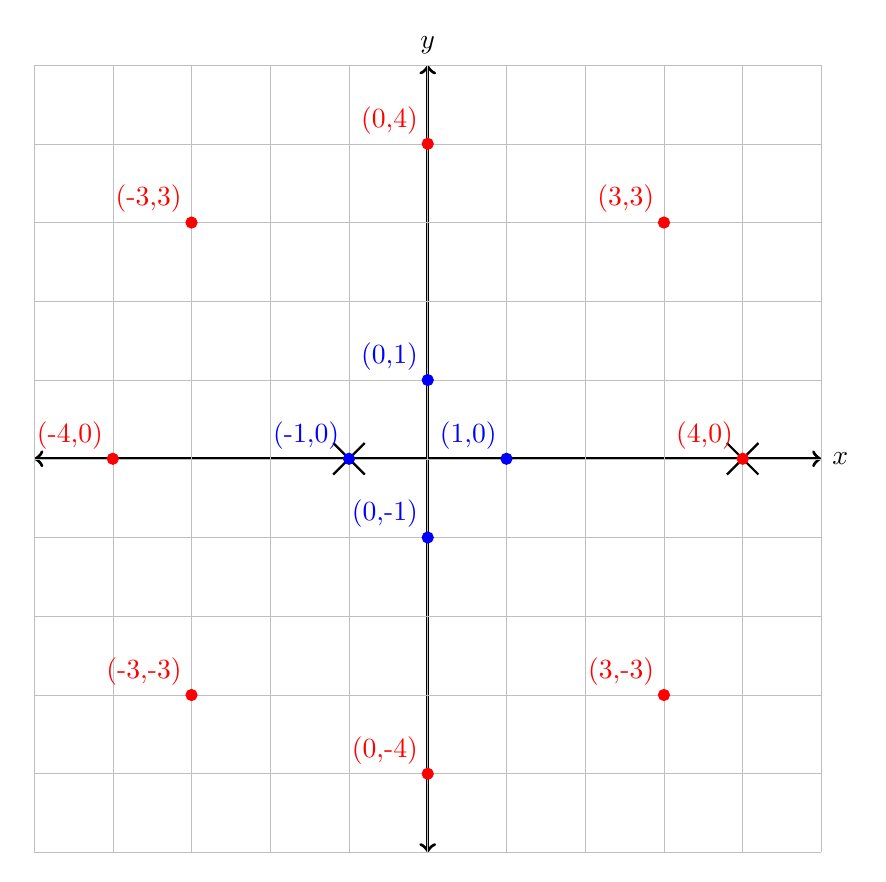
\begin{tikzpicture}
					% Draw the axes with thicker lines
					\draw[<->, very thick] (-5,0) -- (5,0) node[right] {$x$};
					\draw[<->, very thick] (0,-5) -- (0,5) node[above] {$y$};
					
					% Draw faded grid
					\draw[step=1cm,gray!50,very thin] (-5,-5) grid (5,5);
					\draw[thick] (3.8, -0.2) -- (4.2, 0.2);
					\draw[thick] (3.8, 0.2) -- (4.2, -0.2);
					\draw[thick] (-.8, -0.2) -- (-1.2, 0.2);
					\draw[thick] (-.8, 0.2) -- (-1.2, -0.2);
					% Plot the points
					\filldraw[red] (3, -3) circle (2pt) node[anchor=south east] {(3,-3)};
					\filldraw[red] (3, 3) circle (2pt) node[anchor=south east] {(3,3)};
					\filldraw[red] (-3, -3) circle (2pt) node[anchor=south east] {(-3,-3)};
					\filldraw[red] (-3, 3) circle (2pt) node[anchor=south east] {(-3,3)};
					\filldraw[blue] (1, 0) circle (2pt) node[anchor=south east] {(1,0)};
					\filldraw[blue] (0, 1) circle (2pt) node[anchor=south east] {(0,1)};
					\filldraw[blue] (-1, 0) circle (2pt) node[anchor=south east] {(-1,0)};
					\filldraw[blue] (0, -1) circle (2pt) node[anchor=south east] {(0,-1)};
					\filldraw[red] (4, 0) circle (2pt) node[anchor=south east] {(4,0)};
					\filldraw[red] (0, 4) circle (2pt) node[anchor=south east] {(0,4)};
					\filldraw[red] (-4, 0) circle (2pt) node[anchor=south east] {(-4,0)};
					\filldraw[red] (0, -4) circle (2pt) node[anchor=south east] {(0,-4)};
				\end{tikzpicture}
			\end{center}
				\caption{Non-globular Data Points}
				\label{ck}
		\end{figure}
		\begin{figure}[H]
			\begin{center}
				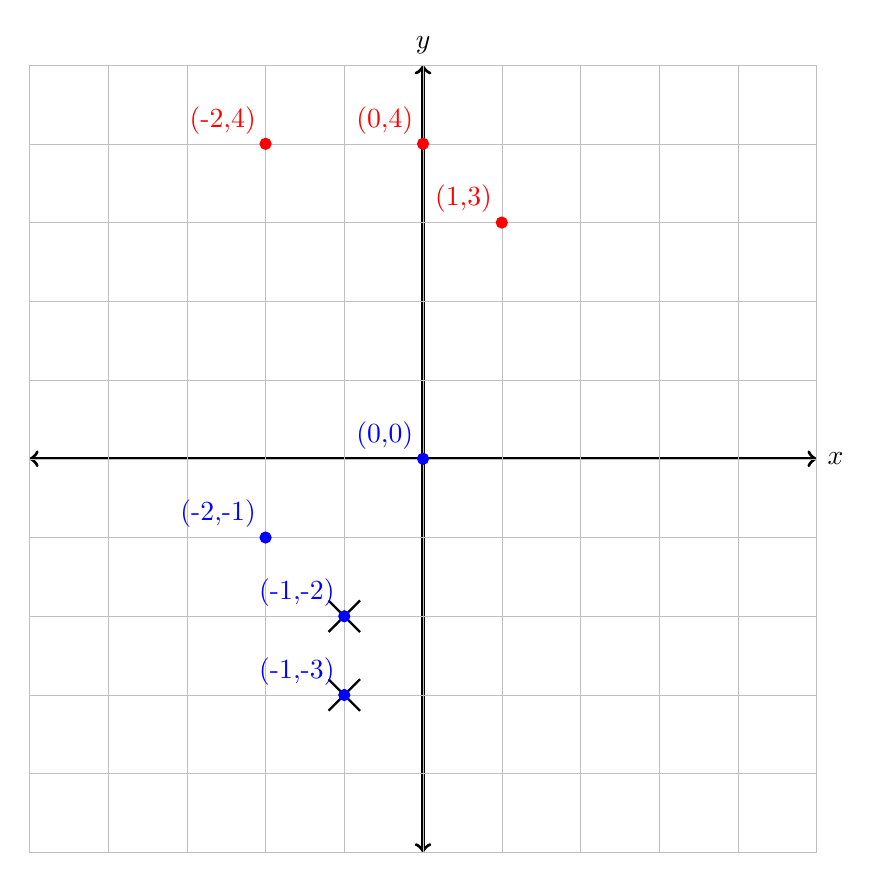
\begin{tikzpicture}
					% Draw the axes with thicker lines
					\draw[<->, very thick] (-5,0) -- (5,0) node[right] {$x$};
					\draw[<->, very thick] (0,-5) -- (0,5) node[above] {$y$};
					
					% Draw faded grid
					\draw[step=1cm,gray!50,very thin] (-5,-5) grid (5,5);
					
					% Plot the points
					\draw[thick] (-1.2, -3.2) -- (-.8, -2.8);
					\draw[thick] (-1.2, -2.8) -- (-.8, -3.2);
					\draw[thick] (-1.2, -2.2) -- (-0.8, -1.8);
					\draw[thick] (-1.2, -1.8) -- (-0.8, -2.2);
					\filldraw[red] (0, 4) circle (2pt) node[anchor=south east] {(0,4)};
					\filldraw[red] (1, 3) circle (2pt) node[anchor=south east] {(1,3)};
					\filldraw[blue] (-1, -3) circle (2pt) node[anchor=south east] {(-1,-3)};
					\filldraw[blue] (-2, -1) circle (2pt) node[anchor=south east] {(-2,-1)};
					\filldraw[blue] (0, 0) circle (2pt) node[anchor=south east] {(0,0)};
					\filldraw[blue] (-1, -2) circle (2pt) node[anchor=south east] {(-1,-2)};
					\filldraw[red] (-2, 4) circle (2pt) node[anchor=south east] {(-2,4)};
				\end{tikzpicture}
			\end{center}
			\caption{Globular Data Points}
			\label{bk}
		\end{figure}
		\newpage
	\part{Practical Assignment:\\Agglomerative Clustering}
	\section*{Task}
	In this exercise, you'll manually perform agglomerative clustering with centroid linkage on a given set of 7 data points. Your tasks include calculating a proximity matrix, performing the clustering steps, constructing a dendrogram, and visually representing the clustering on a 2D grid. Finally, analyze the dendrogram to determine and justify the best number of clusters.
	\section*{Data Points}
	\begin{figure}[H]
		\begin{center}
				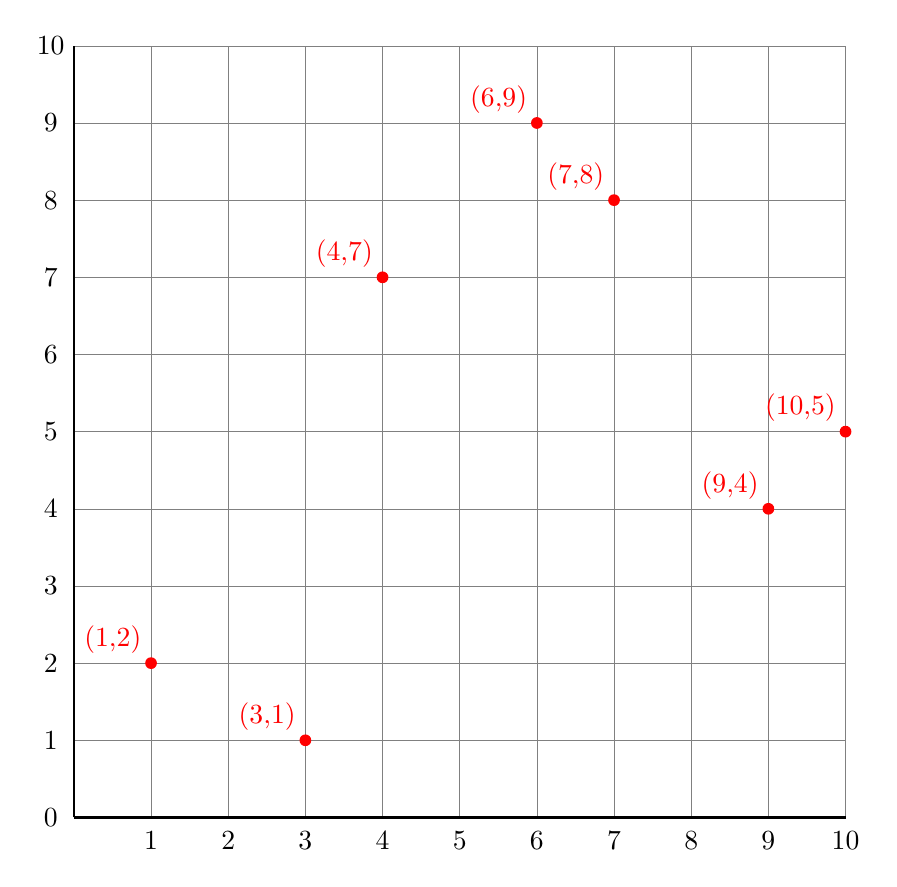
\begin{tikzpicture}[scale=.98]
					% Draw grid
					\draw[step=1cm,gray,very thin] (0,0) grid (10,10);
					
					% Draw axes
					\draw[thick] (0,0) -- (0,10);
					\draw[thick] (0,0) -- (10,0);
					
					% Label axes
					\foreach \x in {1,...,10} \node at (\x,-0.3) {\x};
					\foreach \y in {0,1,...,10} \node at (-0.3,\y) {\y};
					
					% Plot data points
					\node at (1,2) [circle,fill=red,inner sep=1.5pt] {};
					\node at (4,7) [circle,fill=red,inner sep=1.5pt] {};
					\node at (10,5) [circle,fill=red,inner sep=1.5pt] {};
					\node at (3,1) [circle,fill=red,inner sep=1.5pt] {};
					\node at (9,4) [circle,fill=red,inner sep=1.5pt] {};
					\node at (7,8) [circle,fill=red,inner sep=1.5pt] {};
					\node at (6,9) [circle,fill=red,inner sep=1.5pt] {};
					
					% Label data points
					\node[above left,red] at (1,2) {(1,2)};
					\node[above left,red] at (4,7) {(4,7)};
					\node[above left,red] at (10,5) {(10,5)};
					\node[above left,red] at (3,1) {(3,1)};
					\node[above left,red] at (9,4) {(9,4)};
					\node[above left,red] at (7,8) {(7,8)};
					\node[above left,red] at (6,9) {(6,9)};
				\end{tikzpicture}
		\end{center}
		\caption{Agglomerative Clustering Data Points}
		\label{pr}
	\end{figure}
	\newpage
	\part{Implementation Assignment:\\DBSCAN}
	\section*{Dataset}
			\begin{verbatim}
		import numpy as np
		import matplotlib.pyplot as plt
		np.random.seed(42)
		n = 500
		x_o = np.array([.3,-1,-1.5])
		y_o = np.array([-.6,-1.5,2])
		x_b = np.random.normal(-.25, .1, n//5)
		y_b = np.random.normal(0, .1, n//5)
		theta = np.random.uniform(0, 10, n)
		r = .5 + .15 * theta
		x_s = r * np.cos(theta)
		y_s = r * np.sin(theta) + np.random.normal(0, .1, n)
		x_1 = np.hstack([x_o, x_b, x_s])
		x_2 = np.hstack([y_o, y_b, y_s])
		
		
		# Dataset X
		X = np.vstack([x_1,x_2]).T
		
		
		plt.figure(figsize=(8, 8))
		plt.scatter(X[:,0],X[:,1])
		plt.grid(True)
		plt.show()
	\end{verbatim}
		\section*{Task}
		In this exercise, you will implement the DBSCAN algorithm from scratch and test it on synthesized data. Your goal is to correctly cluster the data by adjusting the DBSCAN parameters and to report the parameters that yield the best clustering results.
	\part{Implementation Assignment:\\Clustering Algorithms and PCA}
	\section*{Task}
		The goal of this assignment is to compare different clustering algorithms, K-means and DBSCAN. You will visualize the results in 2D and 3D using PCA, and determine which algorithm performs best for the given data. You will also evaluate the impact of the number of clusters on K-means and analyze DBSCAN's behavior with respect to high-dimensional data.
%		\begin{enumerate}
%			\item \textbf{K-means}
%		\end{enumerate}
		\subsubsection*{K-means:}
		\begin{enumerate}
			\item Load the Digits Dataset:
			\begin{itemize}
				\item[-] Use the Digits dataset from \textit{sklearn.datasets}.
				\item[-] Preprocess the data by standardizing it (using \textit{standardscaler}) for better clustering performance.
			\end{itemize}
			\item Apply K-means clustering:
			\begin{itemize}
				\item[-] Perform K-means clustering for a range of k values (e.g., 1 to 20).
				\item[-] Plot the inertia (within-cluster sum of squares) for different k values and analyze the elbow method to identify the optimal number of clusters.
			\end{itemize}
			\item Visualize K-means clusters in 2D and 3D using PCA:
			\begin{itemize}
				\item[-] Reduce the data to 2D and 3D using PCA.
				\item[-] In each case, plot the projected points in two side-by-side figures: one where the projected points are colored according to the true labels (ground truth) and the other where they are colored based on the predicted labels using K-means.
			\end{itemize}
		\end{enumerate}
		\subsubsection*{DBSCAN:}
		\begin{enumerate}
			\item Apply DBSCAN clustering.
			\item Experiment with DBSCAN using different values for eps (epsilon) and min\_samples.
			\item Visualize DBSCAN clusters in 2D and 3D using PCA:
			\begin{itemize}
				\item[-] In each case, plot the projected points in two side-by-side figures: one where the projected points are colored according to the true labels (ground truth) and the other where they are colored based on the predicted labels using DBSCAN.
				\item[-] Does DBSCAN perform better than K-means or not? Explain why.
			\end{itemize}
		\end{enumerate}
	\section*{Note}
	Any attempt to use AI tools for generating the code is strictly prohibited. Students will be asked to present and explain their code during a class session.
\end{document}
